\section{A Causal-Decoder Arm: Qwen2.5-1.5B with LoRA}
\label{sec:qwen}

The ten systems compared in Section~\ref{sec:results} span classical, recurrent
and bidirectional-encoder paradigms. A fourth paradigm --- the modern
causal-decoder small language model --- was explored separately, and we report
it here rather than in Table~\ref{tab:main} for a reason we make explicit below.

\subsection{Method}

Qwen2.5-1.5B \cite{yang2024qwen2} was adapted for nine-way classification with
Low-Rank Adaptation \cite{hu2021lora}: rank $r=16$, $\alpha=32$, dropout $0.05$,
applied to all attention and MLP projections
(\texttt{q,k,v,o,gate,up,down\_proj}) with the classification head left
trainable. This updates roughly $1.2\%$ of the 1.54B backbone. Training used
class-weighted cross-entropy, AdamW at $2\times10^{-4}$ with linear warmup over
the first $10\%$ of steps, batch size 16 with two-step gradient accumulation,
\texttt{bfloat16} autocast, and two epochs. Sequences were truncated to 256
WordPiece-equivalent tokens, matching the BERT arm. Because Qwen is a causal
decoder, the sequence representation is pooled at the last non-padding position,
so padding is applied on the right and \texttt{pad\_token\_id} is set explicitly.

\subsection{Why this result is not in the main table}

The run was carried out on a separately prepared copy of the corpus with its own
label mapping, and was scored on a \textbf{5,000-document} test subset rather
than the 303,213-document split used by every other system in this paper. The
training budget for that copy was not recorded, so we cannot confirm it matched
the 200,000-row budget that makes Table~\ref{tab:main} a controlled comparison.
Placing the resulting figure in that table would break the one property the
table exists to guarantee.

The size of the risk is measurable, and it is not negligible. Using the stored
test predictions of three of our own models, we resampled 5,000-document subsets
of the real test split 30 times and recomputed macro F1 (Table~\ref{tab:subset}).
A subset drawn \emph{proportionally} to the true class priors is essentially
unbiased, but carries a standard deviation of about $1.1$ points --- wider than
the margin separating most adjacent rows of Table~\ref{tab:main}. A
\emph{class-balanced} subset of the same size inflates macro F1 by roughly six
points, because the rare classes whose precision collapses under a $52.9{:}1$
prior are no longer rare.

\begin{table}[t]
\centering
\small
\begin{tabular}{lccc}
\toprule
\textbf{Model} & \textbf{Full} & \textbf{Prop. 5k} & \textbf{Bal. 5k} \\
\midrule
BERT Base           & 0.7647 & $0.766 \pm 0.011$ & $0.824 \pm 0.005$ \\
Logistic Regression & 0.7367 & $0.739 \pm 0.007$ & $0.810 \pm 0.005$ \\
Random Forest       & 0.6920 & $0.690 \pm 0.008$ & $0.751 \pm 0.006$ \\
\bottomrule
\end{tabular}
\caption{Test macro F1 on the full 303,213-document split against 5,000-document
subsets, over 30 resamples. Proportional subsets are unbiased but noisy;
class-balanced subsets are inflated by about six points. This is why a
subset-scored result cannot be quoted alongside full-split results.}
\label{tab:subset}
\end{table}

We cannot determine from the recorded artefacts which of the two regimes the
Qwen subset followed. Its normalised confusion matrix (Figure~\ref{fig:qwencm})
implies an accuracy of $0.80$ if the subset was balanced and $0.87$ if it was
proportional, and the reported accuracy of $0.828$ falls between them.

\subsection{Provisional result}

Subject to those caveats, the run reached a macro F1 of approximately $0.74$ and
an accuracy of approximately $0.83$ on its own 5,000-document subset, with a
per-document inference cost roughly an order of magnitude above BERT's --- the
expected consequence of a 1.5B decoder against a 110M encoder. The confusion
structure in Figure~\ref{fig:qwencm} is qualitatively consistent with the
encoder models: \emph{Credit reporting} is recovered most reliably, the
\emph{Debt collection} $\rightarrow$ \emph{Credit reporting} corridor is the
dominant off-diagonal term, and \emph{Payday / personal loan} is the weakest
class. We therefore treat the arm as evidence that a LoRA-adapted decoder is
\emph{competitive} on this task, and not as a measured ranking against the ten
systems in Table~\ref{tab:main}.

\begin{figure}[t]
\centering
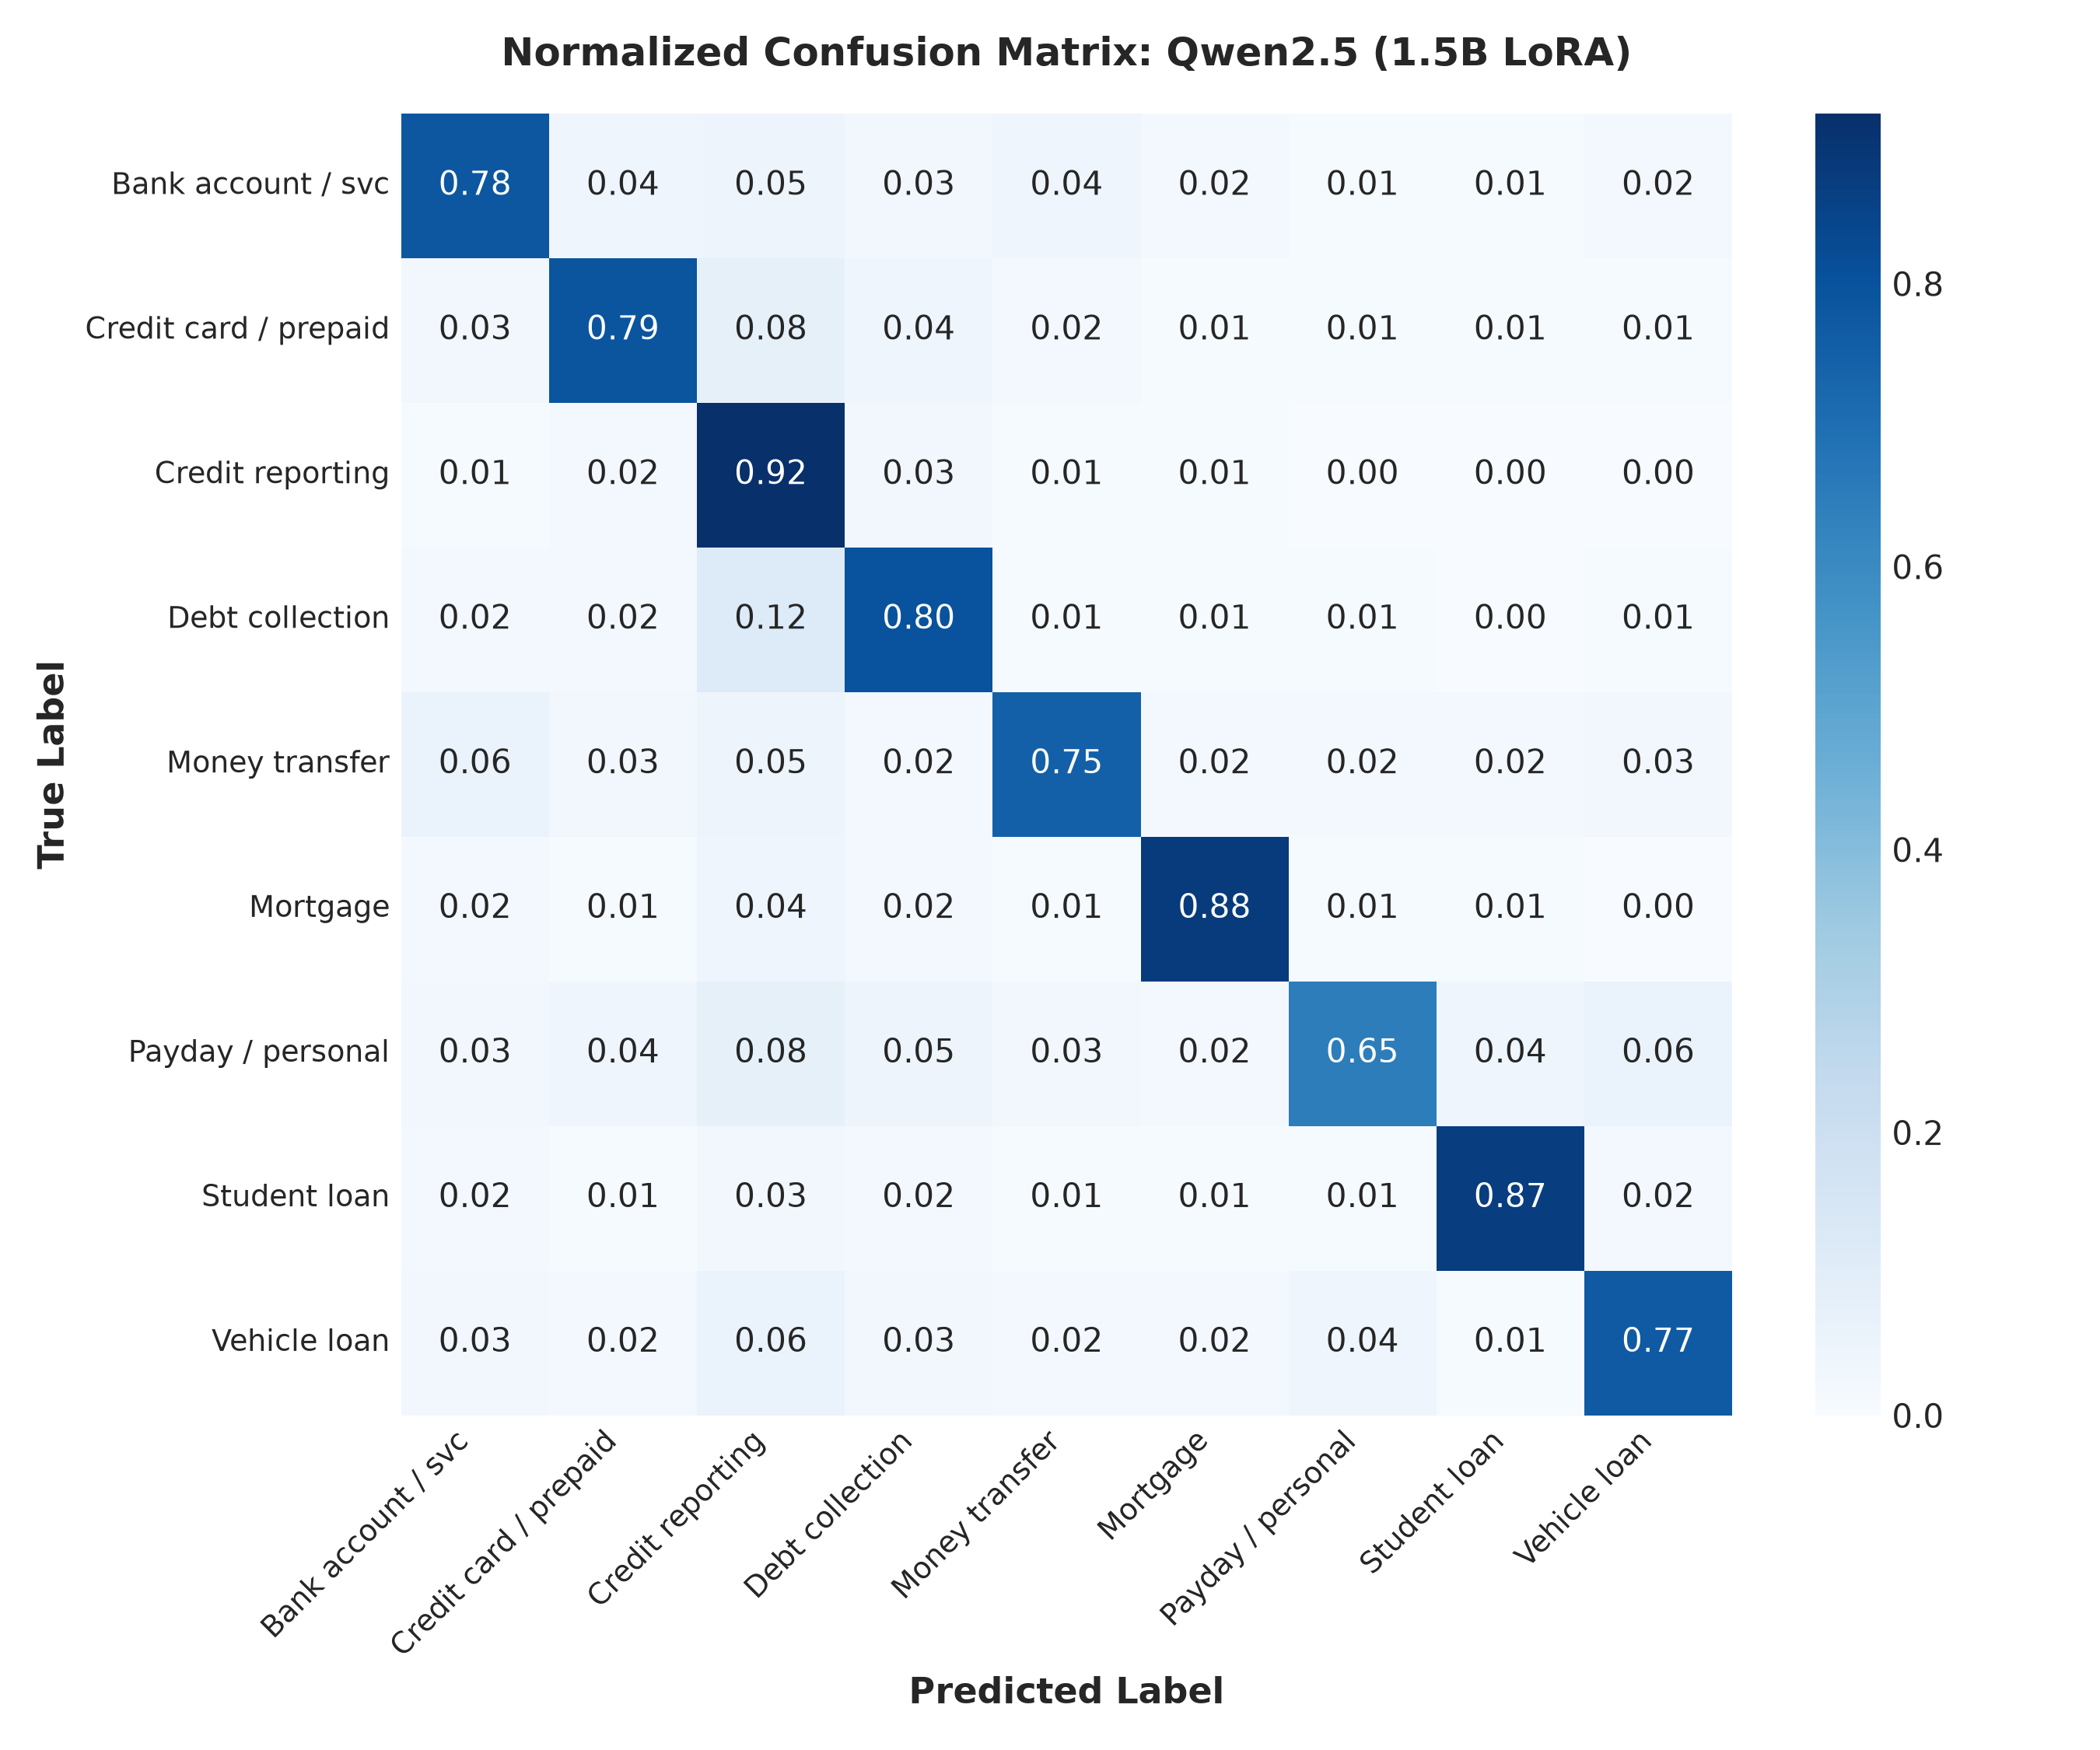
\includegraphics[width=\columnwidth]{figures/qwen_confusion_matrix.png}
\caption{Row-normalised confusion matrix for the Qwen2.5-1.5B LoRA arm on its
5,000-document evaluation subset. Row normalisation makes the diagonal a recall
estimate, which is comparable in shape to the encoder models even though the
scalar metrics are not comparable in level.}
\label{fig:qwencm}
\end{figure}

\subsection{Promoting this arm to the main table}

\texttt{pipeline/qwen\_lora.py} in this repository reproduces the adaptation
above against the shared splits: the same 200,000-row stratified training
budget, the same validation split for epoch selection, and the full
303,213-document test split, with inference timed in the same units as
Table~\ref{tab:main}. Running it writes
\texttt{\_cache/qwen\_lora\_results.json}, including a \texttt{protocol} block
recording the split sizes actually used. Once that file exists, the arm can be
promoted into the main comparison and this appendix retired.
